% begin module differentiable-counterexamples
\begin{frame}
\frametitle{How Can a Function Fail to be Differentiable?}
\begin{columns}[c]
\column{.3\textwidth}
\psset{xunit=1cm, yunit=1cm}
\begin{pspicture}(-0.5,-0.5)(3,2.5)
\psaxes[ticks=none, labels=none]{<->}(0,0)(-0.5,-0.5)(3,2.5)
%Function formula: - (x)+5/2 
\psplot[linecolor=red, plotpoints=1000]{1}{3}{2.5 x -1 mul add } %Function formula: (x)^{2}+1/2 
\psplot[linecolor=red, plotpoints=1000]{-0.2}{1}{0.5 x 2 exp add }
\psline(1,0)(1,0.1) 
\rput[t](1,-0.1){$a$}
\end{pspicture} 
%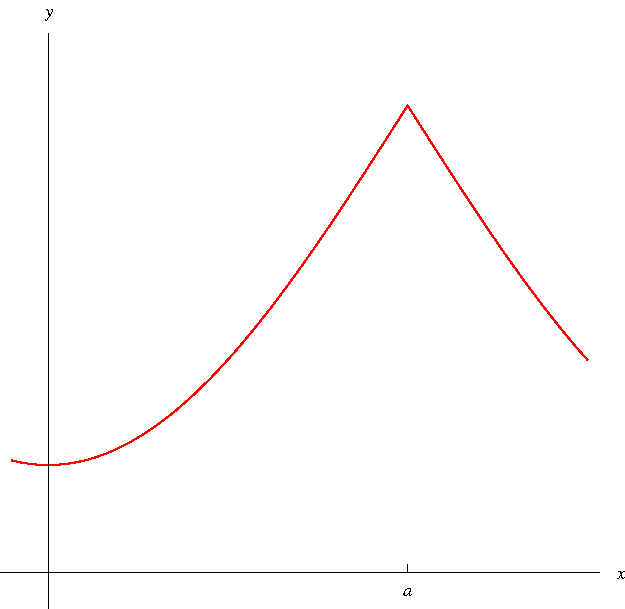
\includegraphics[height=3cm]{derivatives/pictures/03-02-noprimea.pdf}%

\uncover<2->{%
corner
}%
\column{.3\textwidth}
\begin{pspicture}(-0.5,-0.5)(3,2.5)
\psaxes[ticks=none, labels=none]{<->}(0,0)(-0.5,-0.5)(3,2.5)
%Function formula: 1/2+1/2 (x)-1/2 ((x)^{2})+1/8 ((x)^{3}) 
\psplot[linecolor=red, plotpoints=1000]{1}{3}{x 3 exp 0.125 mul x 2 exp -0.5 mul add x 0.5 mul add 0.5 add } %Function formula: x- ((x)^{2})+2 
\psplot[linecolor=red, plotpoints=1000]{-0.2}{1}{2 x 2 exp -1 mul add x add }
\psHollowDot{1}{2}
\psFullDot{1}{0.625}
\psline(1,0)(1,0.1) 
\rput[t](1,-0.1){$a$}
\end{pspicture} 
%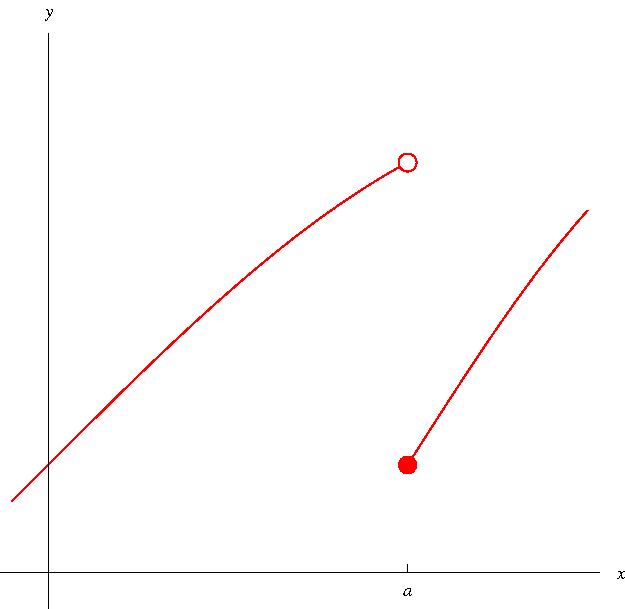
\includegraphics[height=3cm]{derivatives/pictures/03-02-noprimeb.pdf}%
\uncover<3->{%
discontinuity 
}%
\column{.3\textwidth}
\ 
\begin{pspicture}(-0.5,-0.5)(3,2.5)
\psaxes[ticks=none, labels=none]{<->}(0,0)(-0.5,-0.5)(3,2.5)
%Function formula: (-1+x)^{1/3}+1 
\psplot[linecolor=red, plotpoints=1000]{1.00000001}{2.5}{1 x -1 add 0.333333 exp add } %Function formula: - ((- (x)+1)^{1/3})+1 
\psplot[linecolor=red, plotpoints=1000]{0}{0.99999999}{1 1 x -1 mul add 0.333333 exp -1 mul add }
\psline(1,0)(1,0.1) 
\rput[t](1,-0.1){$a$}
\uncover<4>{\psline[linecolor=blue](1,0.2)(1,2.4) }
\end{pspicture} 
%\ \only<handout:0| -3>{%
%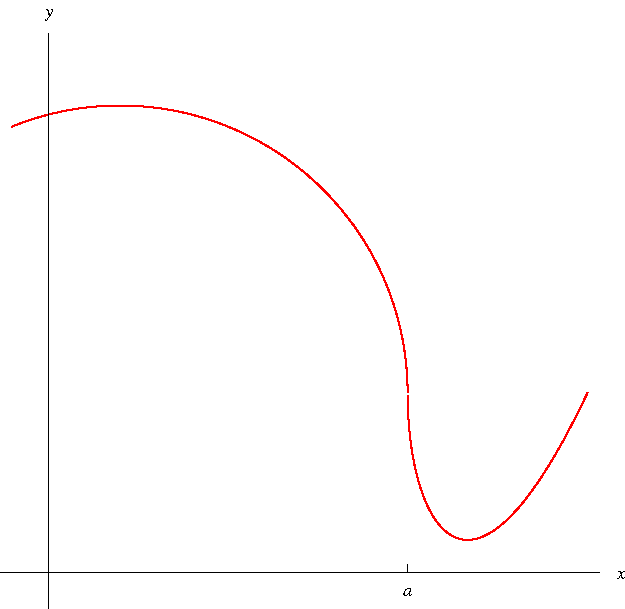
\includegraphics[height=3cm]{derivatives/pictures/03-02-noprimec.pdf}%
%}%
%\only<4->{%
%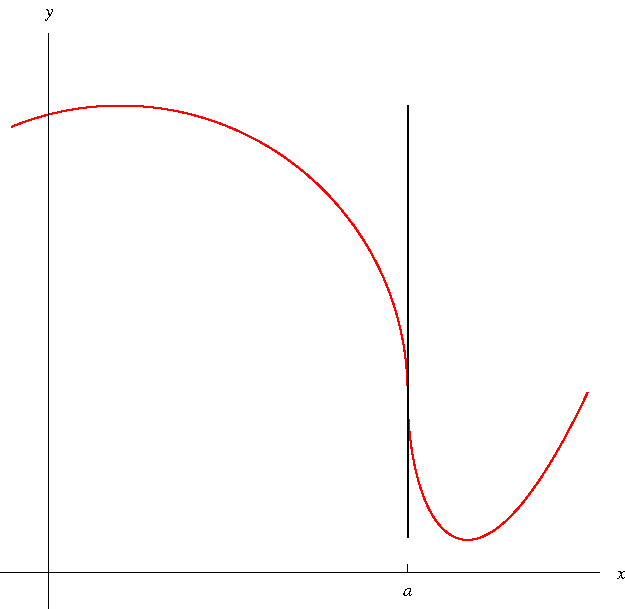
\includegraphics[height=3cm]{derivatives/pictures/03-02-noprimed.pdf}%
%}%
\uncover<4->{%
vertical tangent 
}%
\end{columns}
\end{frame}
% end module differentiable-counterexamples